\chapter{Einleitung}


\chapter{Projektdefinition}
\section{Zielsetzung und Anforderungen}
Das Ziel des Projekts ist es, ein Spiel zu entwickeln, das die Möglichkeiten des Smovetec-Fahrradergometers im Bereich Videospiele demonstriert. Insbesondere ist liegt also der Fokus des Projekts darin, eine Spielidee zu finden, welche die Steuerungsmechanismen Trittfrequenz und Neigung mit einem spaßigen Konzept verbindet.\\
Die wichtigste Anforderung an das Projekt ist also eine sinnvolle Nutzung des Fahrradergometers als Eingabegerät. Da das eingesetzte Fahrradergometer nicht unbedingt immer zur Verfügung steht, ist eine Ersatzsteuerung nur mit Maus und Tastatur sinnvoll.\\
Eine weitere wichtige Anforderung ist außerdem, dass das entstandene Spiel Spaß machen soll. Da das Spiel jedoch vor allem zu Demonstrationszwecken dienen soll, ist es insbesondere wichtig, dass das Spiel nicht kompliziert zu erlernen ist und auch für alle Altersstufen geeignet ist, zumindest im Rahmen der vom Fahrradergometer vorgegebenen Grenzen. Für Kinder unter 6 Jahren wird das Spiel somit vermutlich nicht geeignet sein, da für das Ergometer eine gewisse Körpergröße erforderlich ist.\\
Aus dem Einsatzzweck heraus ergibt sich auch, dass eine längere Bindung von Spielern, wie beispielsweise durch eine Story, ein Highscore-System oder durch einen Mehrspielermodus nicht notwendig ist.\\
Die Zielgruppe ist somit jeder, insbesondere auch ohne Videospiel-Erfahrung, im Alter ab 6 Jahren.\\
\textcolor{red}{Nice-to-haves?}
\section{Features}
\begin{itemize}
\item Steuerung durch Trittfrequenz und Neigung
\item Ersatzsteuerung mit Maus und Tastatur
\item Ansprechende optische Darstellung
\item Langsam steigender Schwierigkeitsgrad
\item Untermalung mit Musik und Geräuschen
\item Verschiedene Designs der Spielumgebung
\end{itemize}


\section{Priorisierung}
Oberste Priorität hat die Steuerung mittels Fahrradergometer. Direkt danach kommen eine ansprechende Präsentation und eine gewisse Zahl an Levels, welche einen gemächlich steigenden Schwierigkeitsgrad abbilden.\\
Die Ersatzsteuerung, Musik und verschiedene Designs gehören eher zu den Features mit niedriger Priorität.

\chapter{Konzept}
Bei dem Spiel handelt es sich um ein Geschicklichkeitsspiel, bei dem der Spieler ein Raumschiff über einen Parcours im Weltall steuern muss. Die Level bestehen aus einer geraden Bahn auf der der Spieler das Raumschiff nach Links und Rechts bewegen kann indem er sich auf dem Ergometer in die jeweilige Richtung lehnt. Zusätzlich muss der Spieler durch Springen Hindernissen auf der Bahn ausweichen. Durch die Veränderung seiner Trittfrequenz erhöht, bzw. verringert der Spieler die Geschwindigkeit des Raumschiffes. Für die Bewältigung eines Levels gibt es eine vorgegebene Zeitspanne innerhalb der das Ziel erreicht werden muss. Die Zeitspanne wird durch den verbleibenden Kraftstoff des Raumschiffs symbolisiert.\\
Das Level gilt als erfolgreich beendet, wenn der Spieler es schafft mit dem Raumschiff innerhalb der vorgegebenen Zeit das Ziel zu erreichen. Läuft die Zeit ab, kollidiert der Spieler mit einem Hindernis oder kommt von der Bahn ab, so hat der Spieler das Level nicht geschafft und muss es wiederholen. Hat der Spieler das Level geschafft, erreicht er automatisch das nächste Level. Es ist nicht vorgesehen, den Spielfortschritt zu speichern, beim nächsten Start des Spiels beginnt er wieder beim ersten Level.
\section{Architektur}
Die Architektur der Software wird grob schon durch die Spieleengine Unity vorgegeben, deren Nutzung Teil der Aufgabenstellung ist. Das Verhalten einzelner Spielobjekte wird von an diese angehängte Skripte gesteuert, wobei vermieden wird, unterschiedliche Kompetenzen im selben Skript zu behandeln, auch wenn es sich um das selbe Objekt handelt.\\
Um den gesamten Zustand des Spiels zu halten, gibt es ein GameManager-Objekt mit einem gleichnamigen Skript, welches in der ersten Szene erzeugt wird und ab da an auch beim Laden einer neuen Szene nicht zerstört wird.\\
Die Eingaben vom Fahrradergometer, also Neigung und Trittfrequenz, werden über ein Smartphone beziehungsweise einen daran angeschlossenen Bluetooth-Sensor verarbeitet und dann über WLAN an den Rechner, auf dem das Spiel läuft, übertragen.\\
Eine detaillertere Beschreibung der Architektur des fertigen Spiels wird im Kapitel \ref{Umsetzung} -- Umsetzung gegeben.

\section{Game Design Document}

\textcolor{red}{\textbf{TODO: Illustration}}

\subsection{Spielobjekte}
Die Spielfigur ist ein Raumschiff, welches sich auf der Bahn bewegen kann. Auf der Bahn befinden sich Hindernisse in Form von Tunnel, Barrikaden und Abgründen. Außerhalb der Bahn befindet sich ebenfalls ein Abgrund.\\
Die Bahn kann auf zwei unterschiedlichen Ebenen verlaufen, wobei der Spieler entweder per Sprung oder Rampe die Ebene wechseln kann.

\subsection{User Interface}
Das User Interface zeigt eine Anzeige für die aktuelle Geschwindigkeit und den verbleibenden Kraftstoff in Form von Rundinstrumenten. Der Fortschritt im aktuellen Level wird als horizontaler Balken am oberen Bildschirmrand dargestellt, der sich mit zunehmender erfolgreich absolvierter Strecke füllt. Außerdem wird die Nummer des Levels, in dem sich der Nutzer aktuellen befindet, angezeigt.

\subsection{Sounds}
Bestimmte Spielsituationen, wie zum Beispiel das Beenden eines Levels, eine Kollision mit einem Hindernis und Springen, werden von entsprechenden und zum Thema des Spiels passenden Geräuscheffekten untermalt. Außerdem wird das Klicken eines Knopfes im Menü auch durch einen Ton an den Spieler rückgemeldet.

\subsection{Steuerung}
Das Spiel wird mit dem \textit{Smovetec} Fahrradergometer gesteuert. Durch die Trittfrequenz wird die Geschwindigkeit des Raumschiffs beeinflusst. Die Neigung des Ergometers hingegen lässt das Raumschiff nach Links oder Rechts lenken. Um mit dem Raumschiff springen zu können, muss der Spieler eine Taste am Griff des Ergometers betätigen. Eine weitere Taste lässt den Spieler das aktuelle Level unmittelbar neu starten.

\subsection{Levels}
Es gibt eine feste Anzahl von Levels. Mit dem Erreichen eines höheren Levels steigt auch der Schwierigkeitsgrad und neue Elemente werden schrittweise eingeführt. Die Level befinden sich in verschiedenen Umgebungen, was man anhand der veränderten Hintergründe und Texturen erkennt, sich aber nicht auf das Verhalten des Spiels auswirkt.
\section{Hardware}
\subsection{Smovetec}
Bei dem Smovetec-System handelt es sich um eine Plattform, durch welche man Fahrradergometer horizontal beweglich machen kann. Dadurch kann man das Kurvenfahren mit einem echten Fahrrad sowie den Wiegetritt simulieren. Es eignet sich somit nicht nur für das übliche Konditionstraining, sondern auch zum Training von Balance und Geschicklichkeit.\\
Es können verschiedene Ergometer auf der Plattform festgeschraubt werden, wodurch man in der Wahl des Ergometers freigestellt ist.
\begin{figure}[ht]
\centering
\begin{subfigure}{.4\textwidth}
\centering
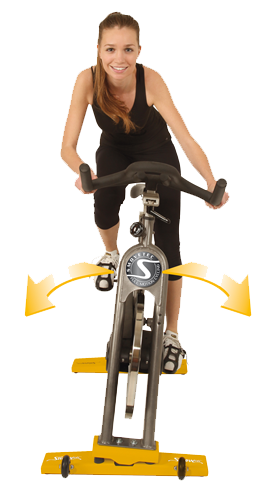
\includegraphics[width=.8\textwidth]{gfx/smovetec.png}
\caption{Das Smovetec-System im Einsatz}
\end{subfigure}
\begin{subfigure}{.59\textwidth}
\centering
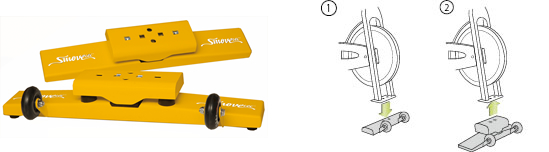
\includegraphics[width=.8\textwidth]{gfx/smovetec2.jpg}
\caption{Das Smovetec-System ohne Ergometer}
\end{subfigure}
\caption{Das Smovetec-System\footnotemark}
\end{figure}
\footnotetext{Quelle: \url{http://www.smovetec.de/smovetec-produkt.htm}}

\subsection{Texas Instruments SensorTag}
Das Smovetec-System selbst ist nicht mit Sensoren ausgestattet um Trittfrequenz oder Neigung zu messen. Um die Trittfrequenz zu messen, kommt in diesem Projekt ein \textit{SensorTag} der Firma Texas Instruments zum Einsatz. Hierbei handelt es sich um ein Bluetooth-fähiges Gerät, welches mit verschiedenen Sensoren ausgestattet ist. Diese umfassen:
\begin{itemize}
\item Temperatursensor
\item Feuchtigkeitssensor
\item Barometer
\item Beschleunigungssensor
\item Gyroskop
\item Magnetometer
\end{itemize}
Für unser Projekt wird davon ausschließlich der Beschleunigungssensor genutzt.\\
Um die Daten auszulesen, kommt eine erweiterte Version der Beispielapp von Texas Instruments zum Einsatz, welche insbesondere auch noch die Beschleunigungssensoren des Smartphones nutzt, um die Neigung zu erfassen. Die Daten werden vom Smartphone per WLAN weiter an den Rechner übermittelt, der das Spiel ausführt.
\begin{figure}[ht]
\centering
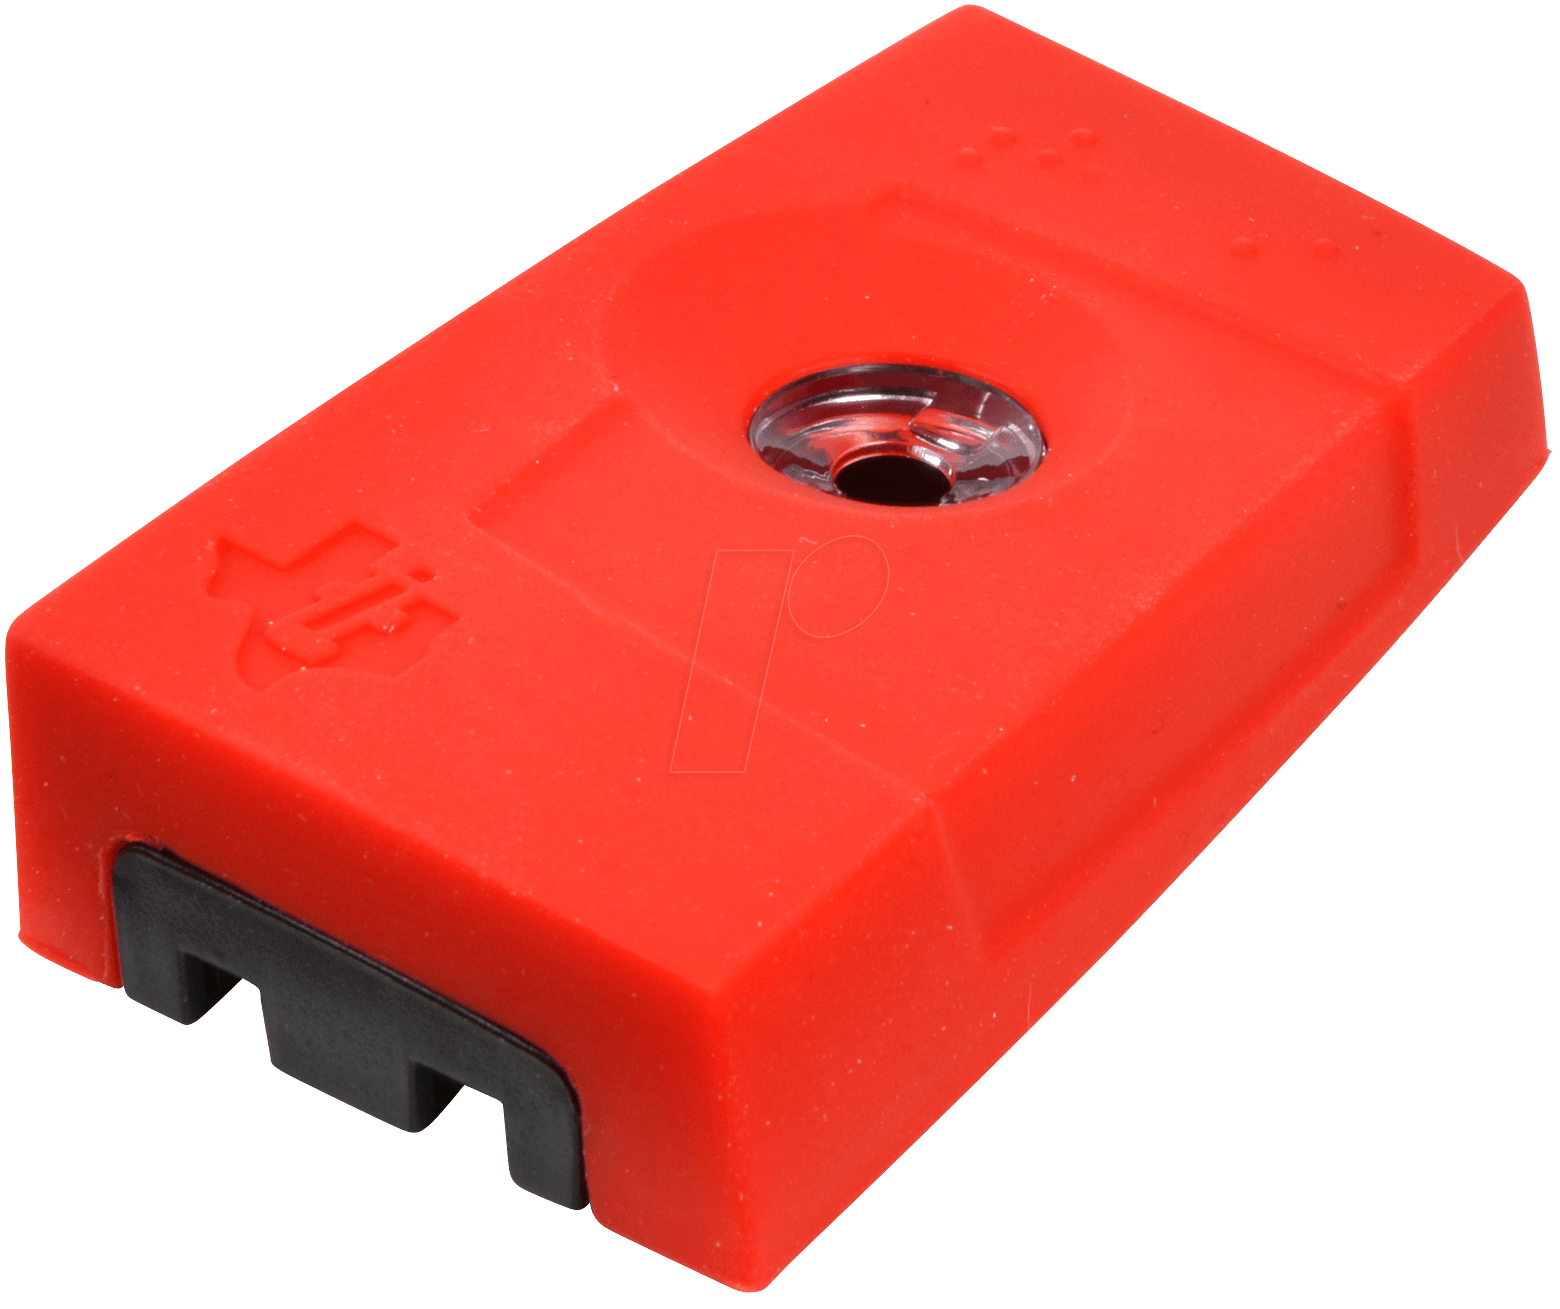
\includegraphics[width=.5\textwidth]{gfx/sensortag.png}
\caption{Texas Instruments SensorTag}
\end{figure}

% \section{Werkzeuge und Technologien}
 
\chapter{Recherche}
\section{Ähnliche Spielideen}
\subsection{Skyroads}
Bei dem Spiel \textit{Skyroads} von \textit{Bluemoon} ist eine Art Jump and Run Spiel aus dem Jahr 1993. Ziel des Spiels ist es ein Raumschiff durch einen Parcour zu manövrieren. Der Spieler muss hierbei über Hindernisse oder Abgründe springen, beziehungsweise diesen ausweichen. Schafft er das Level nicht, kann er es beliebig oft neu starten. Das Prinzip des Spiels stammt aus dem Spiel \textit{Kosmonauts}, welches von den gleichen Entwicklern bereits im Jahre 1989 veröffentlicht wurde. Zu Beginn des Spiels stehen dem Nutzer bereits alle Levels zur Verfügung. Er kann in einer Übersichtsseite das gewünschte Level auswählen. \\
Mit \textit{Skyroads XMAS-Special} wurde 1994 ein Nachfolger veröffentlicht. Außerdem existieren mittlerweile sehr viele andere Spiele, die nach einer ähnlichen Spielmechanik funktionieren.
\begin{figure}[ht]
	\centering
	\begin{subfigure}{6 cm}
	\centering
			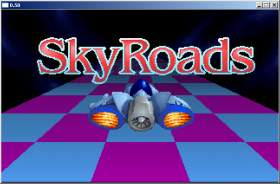
\includegraphics{gfx/recherche/skyroads1.jpg}
	\end{subfigure}
	\begin{subfigure}{6 cm}
	\centering
			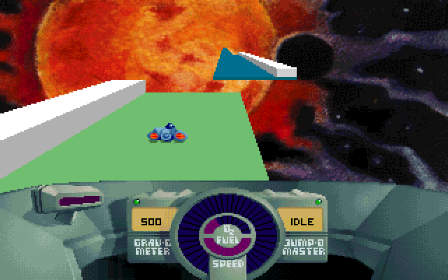
\includegraphics{gfx/recherche/skyroads2.jpg}  
	\end{subfigure}
	\caption{Skyroads}
\end{figure}\\

\subsection{Audiosurf}

Das Geschicklichkeitsspiel \textit{Audiosurf} des Entwicklers \textit{Invisible Handlebar} aus dem Jahr 2008 ist ebenfalls ein Beispiel für eine vergleichbare Spielidee. Auch hier steuert der Spieler ein raumschiffartiges Gefährt über Bahnen und muss dabei Hindernissen ausweichen. Die Besonderheit dieses Spiels ist jedoch, wie der Name andeutet, dass die Strecken automatisch passend zu einem Musikstück generiert werden, das während des Spiels passend dazu abgespielt wird.\\
Je nach Spielmodus muss der Spieler farbige Blöcke auf den Bahnen einsammeln oder grauen Blöcken ausweichen. Die Blöcke werden dann als Rechtecke in einem Raster am unteren Bildschirmrand angesammelt, jeweils auf der Bahn, auf der sie eingesammelt wurden. Sobald drei oder mehr Blöcke gleicher Farbe aneinander angrenzen, blinken diese für wenige Sekunden und lösen sich dann auf, wobei der Spieler dafür Punkte erhält.\\
Ziel des Spiels ist es, auf diese Weise auf jeder Strecke bzw. jedem Lied möglichst viele Punkte zu sammeln. Diese Punkte werden dann auch in einer lokalen und globalen Highscore-Liste eingetragen. Eine weitere Motivation bieten verschiedene Bonusregelungen und Herausforderungen, wie beispielsweise. das Abschließen einer Strecke ohne dass sich am Ende noch Blöcke im Raster befinden oder die Strecke zu beenden ohne einen einzigen grauen Block berührt zu haben.\\
\begin{figure}[ht]
\centering
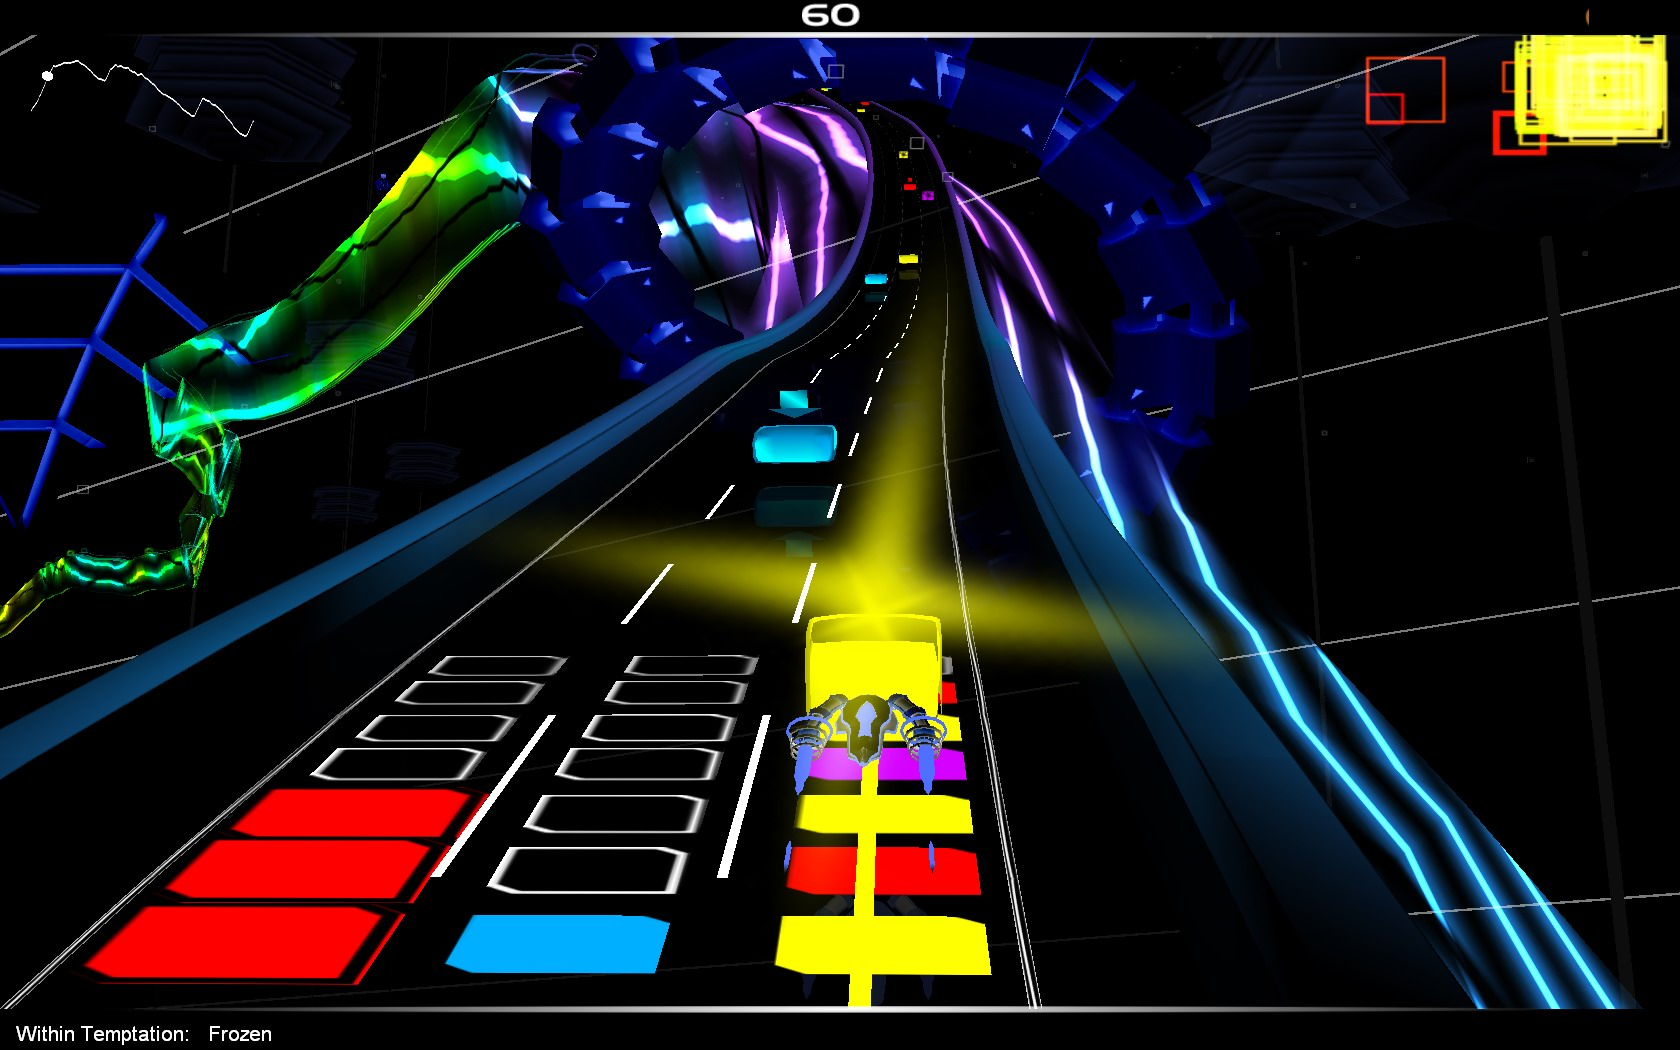
\includegraphics[width=.7\textwidth]{gfx/recherche/audiosurf.jpg}
\caption{Screenshot einer typischen Szene in Audiosurf\footnotemark}
\end{figure}
\footnotetext{Quelle: \url{https://market.myo.com/app/5474d1c6e4b081c4011c77b4/audiosurf-connector}}Ähnlich wie bei unserem Spiel handelt es sich also bei \textit{Audiosurf} um ein Geschicklichkeitsspiel, bei dem man ein Gefährt auf Bahnen hin- und herbewegt um Hindernissen auszuweichen. Anders ist jedoch vor allem, dass es bei \textit{Audiosurf} nicht darum geht, ein Level überhaupt zu schaffen, sondern die Motivation für den Spieler über ein Punkte- und Highscore-System generiert wird. Das wird auch dadurch deutlich, dass es in \textit{Audiosurf} nicht möglich ist, ein Level gar nicht zu schaffen. Kollisionen mit Hindernissen oder ein Überlaufen des Rasters führen hingegen nur zu einem Punktabzug, stören aber sonst nicht den Spielablauf.


\section{Spiele mit Fahrradergometern}
\label{StateOfTheArt}
\subsection{Atari Puffer}
Der 1982 von Atari entwickelte \textit{Atari Puffer} (Abb \ref{ataripuffer}) \cite{Sinclair:2007:CDE:1321261.1321313} war das erste System, welches die Möglichkeit bieten
sollte Videospiele mit dem Körper zu steuern. Plan war es eine Art Fahrradergometer an den \textit{Atari} 					anzuschließen um somit die Spiele zu steuern. Eine erhöhte Umdrehungszahl der Pedale sollte dafür sorgen,
dass zum Beispiel das Auto des Spielers im Spiel \textit{Pole Position} schneller fuhr oder der Spieler im Spiel
\textit{Dig-Dug} schneller gräbt. Zusätzlich konnte ein Gamepad am Lenker montiert werden um zusätzliche
Eingaben zu ermöglichen.\\
Auf Grund der Videospielkrise im Jahr 1984 kam es jedoch nie zur Markteinführung.\\
\begin{figure}[h]
	\centering
	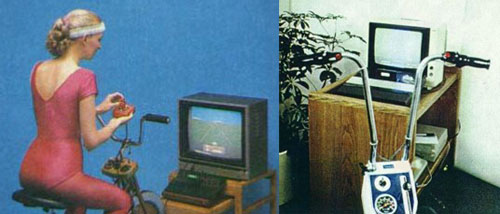
\includegraphics[width=7cm]{gfx/recherche/ataripuffer.jpg} 
		\caption{Atari Puffer}
	\label{ataripuffer}
\end{figure}


\subsection{Thera Trainer}
Die Firma \textit{medica Medizintechnik GmbH} entwickelt, neben dem \textit{Balance-Trainer}, verschiedene Geräte und Programme zur Unterstützung der Bewegungstherapie. Mögliche Anwendungszwecke sind beispielsweise die Therapie von Schlaganfällen, sowie von Muskel- und rheumatischen Erkrankungen. Es findet jedoch auch Anwendung auf dem Gebiet der Orthopädie und Kardiologie. Hierzu bietet der Hersteller verschiedene Trainingsgeräte in Form von Ergometern und Balance Plattformen.\\
\begin{figure}[ht]
	\centering
	\begin{subfigure}{6 cm}
	\centering
			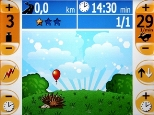
\includegraphics{gfx/recherche/Igel.jpg}
			\caption{Igel}
			\label{Igel}
	\end{subfigure}
	\begin{subfigure}{6 cm}
	\centering
			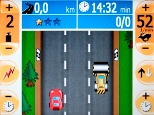
\includegraphics{gfx/recherche/Auto.jpg}  
			\caption{Auto}
			\label{Auto}
	\end{subfigure}
	\caption{Thera Trainer}
\end{figure}\\
Auf dem am Gerät montierten Bildschirm können verschiedene optische Feedbacksysteme angezeigt werden:

\paragraph{Igel:}\noindent
Durch unterschiedliche Kraftverteilung des linken und rechten Beins bewegt sich der Igel in die entsprechende Richtung. Herab fallende Gegenstände sollen dadurch zum platzen gebracht werden. (Abb.~\ref{Igel})

\paragraph{Auto:}\noindent
Der Patient sieht eine Fahrbahn, sowie sein eigenes Fahrzeug. Ziel ist es möglichst viele andere Fahrzeuge zu überholen. Hierzu muss er schneller Treten als eine voreingestellte Drehzahl. Durch Veränderung der Kraftverteilung (siehe \textit{Igel}) kann das Auto nach links und rechts bewegt werden. (Abb.~\ref{Auto})

\subsection{Jeff Sinclaire - Edith Cowan University}
\begin{figure}[ht]
	\centering
	\begin{minipage}[b]{6 cm}
		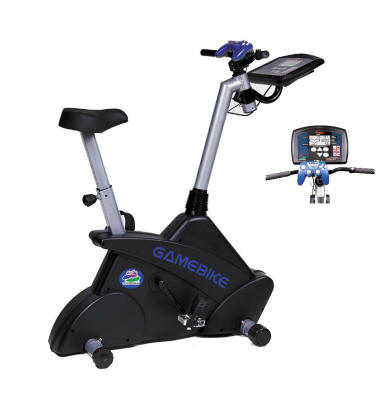
\includegraphics[width=5cm]{gfx/recherche/cateye.jpg} 
			\caption{CatEye GameBike}
			\label{gamebike}
	\end{minipage}
	\begin{minipage}[b]{6 cm}
			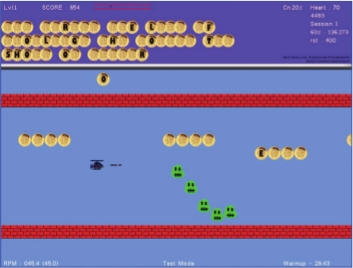
\includegraphics[width=5cm]{gfx/recherche/edith.jpg}  
			\caption{Side Scroller}
			\label{sidescroller}
	\end{minipage}
\end{figure}\noindent
Bei dem Exergaming Projekt der \textit{Edith Cowan University Perth} \cite{5716909} handelt es sich um einen einfachen Side-Scroller, der mit einem Fahrradergometer gesteuert wird (Abb. \ref{sidescroller}). Ziel des Spiels ist es einen Hubschrauber in der richtigen Höhe zu halten und dabei Gegenstände einzusammeln, Hindernissen auszuweichen und Gegner abzuschießen. Je schneller der Spieler tritt, desto höher fliegt der Helikopter. Verringert der Spiele die Geschwindigkeit verliert der Helikopter an Höhe.\\
Als Ergometer kommt hierbei das \textit{GameBike} der Firma \textit{CatEye} (Abb. \ref{gamebike}) zum Einsatz. Das Ergometer kann an die gängigsten, auf dem Markt erhältlichen Spielekonsolen angeschlossen werden und funktioniert mit sämtlichen Spielen, die auf Geschwindigkeit basieren. Für das Projekt der Universität Perth wurde eine Modifikation vorgenommen um es auch an einen PC anschließen zu können.


\subsection{Ergo Active}
Entwickelt wurde \textit{Ergo Active} an der \textit{Technischen Universität Darmstadt} \cite{Gobel:2010:SGH:1873951.1874316} zur Förderung von Serious Games for Health mit wissenschaftlichem Hintergrund, in Bezug auf Sport und Gesundheit. Es umfasst drei Spiele \textit{Taubenjagd, Film} und \textit{Balance} zum Ausdauer-, beziehungsweise Herz-Kreislauftraining. Gesteuert werden alle drei Spiele mittels eines Fahrradergometers.

\paragraph{Taubenjagd:}\noindent
Hierbei handelt es sich um einen einfachen Sidescroller. Der Spieler steuert eine Brieftaube mit Hilfe des Fahrradergometers. Ziel ist es vorbei fliegende Briefe einzusammeln um Punkte zu bekommen. Um so schneller er tritt, desto höher fliegt die Taube. Der Spieler tritt dabei innerhalb eines vorher festgelegten Geschwindigkeit Intervalls, wodurch einerseits verhindert wird, dass der jeweilige Spieler ausserhalb seiner körperlichen Möglichkeiten trainiert und andererseits ein Adaptionsmechanismus für verschiedene Spieler gegeben ist. 

\paragraph{Film:}\noindent
\textit{Film} ermöglicht dem Spieler zum Beispiel Etappen der \textit{Tour de France nachzufahren}. Hierfür wird ein Film der jeweiligen Strecke gezeigt. Je nach dem wie schnell der Spieler Tritt um so schneller wird der Film der jeweiligen Etappe abgespielt. Ähnlich wie bei Taubenjagd findet auch hier eine Überwachung des Spielers statt. Über-, oder unterschreitet er seine Leistungsgrenzen gibt das Spiel ein Signal um den Spieler daraufhin zuweisen wieder innerhalb seines persönlichen Intervalls zu trainieren.

\paragraph{Balance:}\noindent
Bei \textit{Balance} hat der Spieler zwei Aufgaben. Er balanciert einen Clown auf einem Ball. Hierzu muss er mittels Ergometer eine vorgegebene Geschwindigkeit halten, beziehungsweise darf maximal nur um einen bestimmten Wert davon abweichen. Während er den Clown in der Balance hält fallen Luftballons herab, die er mittels Maus oder Wiimote abschießen muss, um Punkte zu sammeln. Die voreingestellte Geschwindikeit und die maximale Abweichung dienen hierbei zur Überwachung, damit  sich der Spieler innerhalb seiner Leistungsgrenzen bewegt. 
\begin{figure}[ht]
	\centering
	\begin{minipage}[b]{6 cm}
			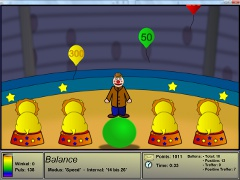
\includegraphics[width=6cm]{gfx/recherche/balance.jpg} 
			\caption{Ergo Active - Balance}
			\label{balance}
	\end{minipage}
	\begin{minipage}[b]{6 cm}
			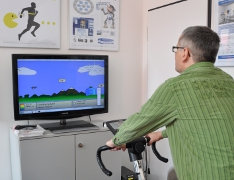
\includegraphics[width=6cm]{gfx/recherche/ergoactive.jpg} 
			\caption{Taubenjagd}
			\label{ergoactive}
	\end{minipage}
\end{figure}

\section{Fazit der Recherche}
In Bezug auf die benutzte Hardware von anderen Systemen, erkennt man, dass Fahrradergometer sehr oft als das bevorzugte Mittel zur Eingabe genutzt werden. Fahrradergometer bieten jedoch nur eine sehr limitierte Bandbreite von möglichen Eingaben. Streng genommen findet man in den betrachteten Systemen ausschließlich zwei Aktionen, die Erhöhung der Trittfrequenz, sowie die Verringerung, beziehungsweise Abbremsen um eine Spielfigur zu steuern und Aktionen einzuleiten \\
Auch in Bezug auf die beanspruchten Körperpartien werden stets nur der untere Teil des Körpers, speziell die Beine, belastet. Einzige Ausnahme sind die Produkte der Firma \textit{medica Medizintechnik GmbH}. Sie bieten ebenfalls Ergometer die mit der Hand und den Armen bedient werden können und sind somit auch, zum Beispiel, für Rollstuhlfahrer geeignet. Alle Systeme jedoch benutzen jeweils nur einen Teil des Körpers zur Eingabe - entweder Beine oder Oberkörper. Keines der betrachteten Systeme bietet die Möglichkeit sowohl Ober- als auch Unterkörper zu aktivieren. \\
Kaum ein System bietet neben der Trittfrequenz, beziehungsweise Geschwindigkeit des Ergometers weitere Eingabeoptionen. Das in unserem Projekt genutzte Ergometer bietet diese Möglichkeit jedoch. Durch die Gewichtsverlagerung mit Hilfe des Oberkörpers können wir in unserem Spiel eine weitere Ebene der Kontrollmöglichkeiten erreichen. Hierdurch wird ermöglicht, dass sich die Spielfigur in diesem Projekt in zwei, statt wie in den anderen Publikationen, nur in einer Dimensionen bewegen kann. Darüber hinaus soll in diesem Projekt eine weitere, dritte Dimension, der Bewegungsfreiheit, das Springen, eingebaut werden. Durch die verschiedenen Aspekte der Steuerung soll die Motivation des Spielers möglichst hoch gehalten werden, da das Spiel vielfältiger ist. Andere Projekte beschränken sich lediglich auf eine mögliche Eingabe, wodurch die Gefahr entsteht, dass das Spiel schnell eintönig und langweilig wird.\\
Trotz der Erweiterten Eingabemöglichkeit dieses Systems im Vergleich zu anderen Projekten, besitzt sie dennoch nicht die volle Bandbreite der möglichen Kommandos, wie es zum Beispiel Spiele bieten, die an einem Stationären Computer mit Tastatur und Maus gesteuert werden. Aus diesem Grund muss das entwickelte Spiel ebenfalls eine einfache, aber interessante, Spielmechanik mit hohem Motivationsfaktor haben. Die beiden betrachteten Spiele \textit{Skyroads} und \textit{Audiosurf} sind hierfür gute Beispiele. Sie kommen jeweils mit verhältnismäßig wenigen Eingaben aus, bieten jedoch trotzdem eine attraktive und motivierende Spielmechanik. Aus diesem Grund sollen diese beiden Spiele eine Art Vorbild für das im Rahmen dieses Praktikums entwickelten Bewegungsspiels darstellen. Ziel wird es sein interessante Konzepte zu Adaptieren, beziehungsweise zu erweitern um die Funktionen des Fahrradergometers möglichst optimal nutzen zu können.


\chapter{Methoden und Vorgehen}
Bei der Durchführung des Projekts hat sich das Team an einem agilen Entwicklungsmodell orientiert. Das bedeutet, dass man nicht zu Beginn eine ausführliche Planung aller Features bis ins Detail durchgeführt hat, sondern, dass vielmehr jede Idee und jeden Ansatz direkt als Mock-up im Spiel ausprobiert wurde, um schnelles und exaktes Feedback über die Machbarkeit und Sinnhaftigkeit des Features zu erlangen.\\
Dieses Vorgehen hat den Effekt, dass manche Features begonnen, aber dann nachdem man festgestellt hat, dass sie so nicht machbar oder nicht zielführend sind, wieder verworfen wurden. Auf der anderen Seite ermöglicht dieses Vorgehen aber auch ein sehr schnelles Reagieren auf neue Begebenheiten. Insbesondere wird so sichergestellt, dass keine überflüssigen Features erst aufwändig geplant werden und sich dann in der Realität als obsolet herausstellen. Aber insbesondere ermöglicht diese Methode ein sehr schnelles Lernen aus Feedback um so ein für den Nutzer optimales Spielerlebnis zu schaffen.\\
\paragraph{Controlling}\noindent
Um den Fortschritt im Projekt und auch mögliche Rückschläge immer möglichst gut im Blick zu behalten, bestreiten wir einen möglichst großen Teil der Entwicklung immer mit dem Team gemeinsam. Wenn dies zeitweise nicht möglich ist, so halten wir uns per E-Mail detailliert auf dem Laufenden. Dennoch ist ein gegenseitiges Update beim nächsten persönlichen Treffen unumgänglich.\\
So oft möglich erfolgt die Entwicklung in den Räumlichkeiten des Lehrstuhls, sodass bei Schwierigkeiten, aber auch für regelmäßiges Feedback der Betreuer unkompliziert hinzugezogen werden kann.
\paragraph{„lessons-learned“}\noindent
Ein genaues Durchführen und Einhalten eines vorab erstellten Plans ist in so einem Softwareprojekt nicht möglich. Gerade wenn man wenig Erfahrung mit den eingesetzten Technologien hat, ist ein Abschätzen der Aufwände nicht einfach und äußerst ungenau. Daher hat es sich am praktikabelsten erwiesen, von Tag zu Tag neu zu priorisieren und zu entscheiden. Trotzdem konnte man das große Ganze immer gut im Blick behalten und man wusste immer in etwa, wo man im Projekt stehen.


\chapter{Planung}
\section{Projektplanung}
\begingroup
\small
\begin{tabularx}{\textwidth}{|X|c|c|c|} \hline
 &  & \multicolumn{2}{c|}{\textbf{Wer?}} \\ \hline
\textbf{Teilobjekte und Arbeitspakete} & \textbf{Summe (Personentage)} & \textbf{Alex} & \textbf{Simon} \\ \hline
\textbf{1. Koordination und Organisation} & \textbf{7} & \textbf{3} & \textbf{4} \\ \hline
1.1. Einrichten der Entwicklungsumgebung & 2 & 1 & 1 \\ \hline
1.2. Einrichten des Dokumentationstemplates & 2 & 1 & 1 \\ \hline
1.3 Einrichten der Repositories & 1 & 0 & 1 \\ \hline
1.4. Zeitplanung & 2 & 1 & 1 \\ \hline
\textbf{2. Konzeption und Findung der Spielidee} & \textbf{7} & \textbf{5} & \textbf{2} \\ \hline
2.1. Findung der Spielidee & 3 & 2 & 1 \\ \hline
2.2. Game Design Document & 2 & 2 & 0 \\ \hline
2.3. Recherche zur Hardware & 2 & 1 & 1 \\ \hline
\textbf{3. Recherche} & \textbf{8} & \textbf{5} & \textbf{3} \\ \hline
3.1. Ähnliche Spielideen recherchieren & 2 & 1 & 1 \\ \hline
3.2. Spiele mit ähnlichen Eingabegeräten recherchieren & 4 & 3 & 1 \\ \hline
3.3. Geeignete Werkzeuge und Technologien & 2 & 1 & 1 \\ \hline
\textbf{4. Entwicklung des Spielgrundgerüsts} & \textbf{7} & \textbf{4} & \textbf{3} \\ \hline
4.1. Rudimentäres Leveldesign & 2 & 1 & 1 \\ \hline
4.2. Einfache Steuerung per Tastatur & 2 & 1 & 1 \\ \hline
4.3. Einfache graphische Darstellung & 2 & 1 & 1 \\ \hline
4.4. Einfaches graphische Benutzerschnittstelle & 1 & 1 & 0 \\ \hline
\textbf{5. Leveldesign} & \textbf{21} & \textbf{9} & \textbf{12} \\ \hline
5.1. Entwicklung eines Levelgesamtkonzepts & 7 & 3 & 4 \\ \hline
5.2. Gestaltung von Grundelementen für die Levels & 6 & 3 & 3 \\ \hline
5.3. Erstellung einer größeren Anzahl Levels & 8 & 3 & 5 \\ \hline
\textbf{6. Steuerung} & \textbf{15} & \textbf{7} & \textbf{8} \\ \hline
6.1. Anbindung der Trittfrequenz & 3 & 1 & 2 \\ \hline
6.2. Anbindung der Fahrradneigung & 8 & 4 & 4 \\ \hline
6.3. Anbindung eines Aktionsbuttons & 4 & 2 & 2 \\ \hline
\textbf{7. Graphische Darstellung} & \textbf{17} & \textbf{9} & \textbf{8} \\ \hline
7.1. Gestaltung von Models und Texturen & 10 & 5 & 5 \\ \hline
7.2. Gestaltung der Spielumgebung & 4 & 2 & 2 \\ \hline
7.3. Gestaltung von Effekten & 3 & 2 & 1 \\ \hline
\textbf{8. GUI} & \textbf{10} & \textbf{4} & \textbf{6} \\ \hline
8.1. Entwicklung eines GUI Konzepts & 2 & 1 & 1 \\ \hline
8.2. Gestaltung der GUI-Elemente & 4 & 1 & 3 \\ \hline
8.3. Implementierung der GUI im Spiel & 4 & 2 & 2 \\ \hline
\textbf{9. Benutzerdokumentation} & \textbf{7} & \textbf{3} & \textbf{4} \\ \hline
\textbf{10. Entwicklerdokumentation} & \textbf{7} & \textbf{4} & \textbf{3} \\ \hline
 &  &  &  \\ \hline
Gesamt & 92 & 46 & 46 \\ \hline
\end{tabularx}

\newenvironment{ganttap}[5]{
\ganttgroup{#1}{2015-#3-#2}{2015-#5-#4} \ganttnewline
}{
\ganttnewline[thick]}


\section{Zeitplanung}
\resizebox{\textwidth}{!}{

\begin{ganttchart}[
x unit=1.2mm,
y unit title=7mm,
y unit chart=7mm,
group label node/.append style={align=left, text width=15em},
bar label node/.append style={align=left, text width=15em},
milestone label node/.append style={align=left, text width=15em},
vgrid={*4{draw=none},*1{dotted},*2{draw=none}},
time slot format=isodate
]{2015-04-22}{2015-09-20}
\gantttitlecalendar{month=shortname} \\
\gantttitle{1}{5}
\gantttitlelist{2,...,22}{7}\\

\ganttmilestone[inline=true]{Milestone 1}{2015-06-21}

\ganttnewline[thick]

\begin{ganttap}{1. Koordination}{22}{04}{29}{04}
\ganttbar{1.1. Zeitplanung}{2015-04-22}{2015-04-26} \ganttnewline
\ganttbar{1.2. Einrichten Template}{2015-04-22}{2015-04-26} \ganttnewline
\ganttbar{1.3. Einrichten Repo}{2015-04-27}{2015-04-29} \ganttnewline
\ganttbar{1.4. Einrichten IDE}{2015-04-27}{2015-04-29}
\end{ganttap}

\begin{ganttap}{2. Konzeption}{22}{04}{29}{04}
\ganttbar{2.1. Spielidee}{2015-04-22}{2015-04-29} \ganttnewline
\ganttbar{2.2. Design Document}{2015-04-22}{2015-04-26} \ganttnewline
\ganttbar{2.3. Recherche Hardware}{2015-04-27}{2015-04-29}
\end{ganttap}

\begin{ganttap}{3. Recherche}{30}{04}{17}{05}
\ganttbar{3.1. Spielideen}{2015-04-30}{2015-05-03} \ganttnewline
\ganttbar{3.2. Eingabegeräte}{2015-05-04}{2015-05-10} \ganttnewline
\ganttbar{3.3. Werkzeuge}{2015-05-11}{2015-05-17}
\end{ganttap}

\begin{ganttap}{4. Spielgrundgerüst}{30}{04}{12}{05}
\ganttbar{4.1. Leveldesign}{2015-04-30}{2015-05-03} \ganttnewline
\ganttbar{4.2. Tastatursteuerung}{2015-04-30}{2015-05-12} \ganttnewline
\ganttbar{4.3. Graphik}{2015-04-30}{2015-05-12} \ganttnewline
\ganttbar{4.4. GUI}{2015-04-30}{2015-05-12}
\end{ganttap}

\begin{ganttap}{5. Leveldesign}{18}{05}{15}{09}
\ganttbar{5.1. Gesamtkonzept}{2015-05-18}{2015-05-24} \ganttnewline
\ganttbar{5.2. Grundelemente}{2015-06-01}{2015-06-14}
\ganttbar{}{2015-07-06}{2015-07-12} \ganttnewline
\ganttbar{5.3. Levelerstellung}{2015-06-15}{2015-06-28}
\ganttbar{}{2015-07-20}{2015-07-26}
\ganttbar{}{2015-08-10}{2015-08-23} \ganttnewline
\ganttbar{5.4. Testen \& Balancing}{2015-06-29}{2015-07-05}
\ganttbar{}{2015-07-27}{2015-08-02}
\ganttbar{}{2015-08-24}{2015-09-13}
\end{ganttap}

\begin{ganttap}{6. Steuerung}{13}{05}{23}{06}
\ganttbar{6.1. Trittfrequenz}{2015-05-13}{2015-05-24} \ganttnewline
\ganttbar{6.2. Neigung}{2015-05-25}{2015-06-14} \ganttnewline
\ganttbar{6.3. Aktionsbutton}{2015-06-15}{2015-06-23}
\end{ganttap}

\begin{ganttap}{7. Gestaltung}{24}{06}{15}{09}
\ganttbar{7.1. Models \& Texturen}{2015-06-24}{2015-07-05}
\ganttbar{}{2015-07-13}{2015-07-26}
\ganttbar{}{2015-08-03}{2015-08-16} \ganttnewline
\ganttbar{7.2. Umgebung}{2015-08-24}{2015-09-06} \ganttnewline
\ganttbar{7.3. Effekte}{2015-09-07}{2015-09-13}
\end{ganttap}

\begin{ganttap}{8. GUI}{29}{06}{19}{07}
\ganttbar{8.1. Konzept}{2015-06-29}{2015-07-05} \ganttnewline
\ganttbar{8.2. Gestaltung}{2015-07-06}{2015-07-19} \ganttnewline
\ganttbar{8.3. Implementierung}{2015-07-06}{2015-07-19}
\end{ganttap}

\ganttgroup{9. Benutzerdokumentation}{2015-08-17}{2015-09-15}
\ganttnewline[thick]
\ganttgroup{10. Entwicklerdokumentation}{2015-04-30}{2015-09-15}


\end{ganttchart}

}
\section{Meilensteine}
\paragraph{Projektdefinition -- 29.4.}
\noindent
Die Projektdefinition enthält die \textit{tabellarische Planung (vgl. \ref{ap1})} des Projektes, das \textit{Gantt-Diagramm (vgl. \ref{ap1})} und das \textit{Game Design Document (vgl. \ref{ap2})}. Ziel ist es, eine erste Übersicht über die Spielidee, den geschätzten Aufwand und die zeitliche Planung des Projektes zu gewinnen.
\paragraph{Mock-up -- 13.5.}
\noindent
Das Mock-up soll dem Projektteam und dem Betreuer eine bereits spielbare Veranschaulichung der Spielidee bieten. Daher enthält dieser Meilenstein das wesentliche \textit{Spielgrundgerüst (vgl. \ref{ap4})}.
\paragraph{Alpha-Version -- 23.6.}
\noindent
Die Alpha-Version soll bereits erahnen lassen, wie das Spiel zu Projektende aussehen soll. Der Umfang ist aber noch sehr eingeschränkt. Zu diesem Meilenstein gehören ein \textit{einfaches Levelpaket (vgl. \ref{ap5})}, die \textit{Steuerung (vgl. \ref{ap6})}, das \textit{Spielermodell und ein einfaches Texturenpaket (vgl. \ref{ap7})}.
\paragraph{Beta-Version -- 19.7.}
\noindent
In der Beta-Version soll das Spiel dann schon alle Elemente enthalten, die es auch in der fertigen Version hat, wenn auch in geringerem Umfang. Daher kommt in dieser Version noch eine \textit{graphische Benutzeroberfläche (vgl. \ref{ap8})} hinzu.
\paragraph{Pre-finale Ausarbeitung -- 2.9.}
\noindent
Die pre-finale Ausarbeitung enthält bereits alle Inhalte der finalen Ausarbeitung, muss aber noch gegebenenfalls überarbeitet werden. Außer den Inhalten der Projektdefinition enthält diese eine \textit{Recherche (vgl. \ref{ap3})}, sowie die \textit{Benutzer- und Entwicklerdokumentation (vgl. \ref{ap9}, \ref{ap10})}.
\paragraph{Finale Version -- 15.9.}
\noindent
Zur finalen Version werden alle noch für das fertige Spiel fehlenden Arbeiten erledigt. Dies beinhaltet ein \textit{vollständiges Levelpaket (vgl. \ref{ap5})} und \textit{vollständige Texturen, Umgebungen und Effekte (vgl. \ref{ap7})}.
\section{Arbeitspakete}
\newcolumntype{Y}{>{\centering\arraybackslash}X}

\newcommand{\aphead}[5]{\begin{tabularx}{\textwidth}{lYr}
\textbf{Beginn:} #1 \hspace{0.5cm} \textbf{Ende:} #2 & \textbf{Lead:} #3 \hspace{0.5cm} \textbf{Beteiligte:} #4 & \textbf{Aufwand:} #5
\end{tabularx}
\hrule}

\subsection{Koordination und Organisation}
\aphead{22.4.}{29.4.}{alle}{alle}{7 Personentage}

\paragraph{Zielstellung}\noindent
Ziel des Arbeitspaketes \textit{Koordination und Organisation} ist es, die Grundlagen für einen erfolgreichen Start des Projektes zu legen. Nach Abschluss des Arbeitspaketes Koordination und Organisation sollen die Gruppenmitglieder in der Lage sein, die Arbeit am eigentlichen Produkt aufnehmen zu können.

\paragraph{Beschreibung}\noindent
Das Arbeitspaket \textit{Koordination und Organisation} gliedert sich in vier Teilobjekte. Im ersten Teilobjekt wird die Zeitplanung des Projektablaufs vorgenommen. Hierfür wird neben einer tabellarischen Gliederung der Arbeitspakete ein Gantt-Diagramm des zeitlichen Ablaufs erstellt.\\
Anschließend werden Templates für das Projektmanagementdokument eingerichtet und angepasst. Dafür, und für den Quellcode des Projekts, werden im dritten Teilobjekt Versionsverwaltungsrepositories mit Git angelegt und eingerichtet. Abschließend beginnen die Projektbeteiligten damit, die nötigen Entwicklungsumgebungen und Tools einzurichten.

\paragraph{Rolle der Beteiligten}\noindent
Da das Arbeitspaket \textit{Koordination und Organisation} für den gesamten Projektablauf entscheidend ist, sind alle Projektmitglieder hier gleichermaßen beteiligt. Dabei ist jedes Mitglied für die Einrichtung seiner Werkzeuge selbst verantwortlich.

\paragraph{Deliverables}\noindent
\begin{itemize}
\item Tabellarischer Projektplan, Dokument, bis 29.4.
\item Gantt-Diagramm, Dokument, bis 29.4.
\end{itemize}

\paragraph{Meilensteine}\noindent
\begin{itemize}
\item Der \textit{tabellarische Projektplan} und das \textit{Gantt-Diagramm} sind Teil des Meilensteins \textit{Projektdefinition}.
\end{itemize}

\subsection{Konzeption und Findung der Spielidee}
\aphead{22.4.}{29.4.}{Alex}{alle}{7 Personentage}

\paragraph{Zielstellung}\noindent
Ziel des Arbeitspaketes \textit{Konzeption und Findung der Spielidee} ist es, ein Konzept für ein Bewegungsspiel mit einem Fahrradergometer bedient werden soll, zu entwickeln. Außerdem soll ein \textit{Game Design Document}, welches das Konzept genauer erläutert, verfasst werden.

\paragraph{Beschreibung}\noindent
Das Arbeitspaket \textit{Konzeption und Findung der Spielidee} untergliedert sich in drei Teilobjekte. Zunächst erarbeiten die Projektmitglieder eine auf die Aufgabenstellung passende Spielidee. Das gefundene Konzept wird im zweiten Teilobjekt detailliert ausgearbeitet und als \textit{Game Design Document} ausformuliert. Da die bereitgestellte Hardware in Form des Eingabegeräts Fahrradergometer für die Projektbeteiligten unbekannt ist, wird außerdem eine umfassende Recherche zu den technischen Möglichkeiten und Einschränkungen durchgeführt. 

\paragraph{Rolle der Beteiligten}\noindent
Alle Mitglieder des Projektes erarbeiten gemeinsam das Konzept für die Spielidee, sowie die Recherche zur Hardware. Das \textit{Game Design Document} wird überwiegend vom Hauptverantwortlichen des Arbeitspaketes verfasst.

\paragraph{Deliverables}\noindent
\begin{itemize}
\item \textit{Game Design Document}, Dokument, bis 29.4.
\end{itemize}

\paragraph{Meilensteine}\noindent
\begin{itemize}
\item Das \textit{Game Design Document} ist Teil des Meilensteins \textit{Projektdefinition}.
\end{itemize}
\subsection{Recherche}
\aphead{22.4.}{1.9.}{Alex}{alle}{8 Personentage}

\paragraph{Zielstellung}\noindent
Ziel des Arbeitspaketes \textit{Recherche} ist es, eine Übersicht über einige, bereits existierende, Spiele mit vergleichbarer Steuerung beziehungsweise ähnlicher Spielidee zu gewinnen. Außerdem sollen für die Umsetzung des Projektes geeignete Technologien und Werkzeuge gesucht und bewertet werden.

\paragraph{Beschreibung}\noindent
Das Arbeitspaket \textit{Recherche} gliedert sich in drei Teilobjekte, wobei sich die Pakete zur Recherche von ähnlichen Spielideen und Spielen mit ähnlichen Eingabegeräten in ihrer Ausgestaltung überschneiden. Der Fokus der Recherche liegt sowohl auf kommerziellen Produkten, als auch auf wissenschaftlichen Projekten.\\
Nach Abschluss des Arbeitspaketes \textit{Konzeption und Findung der Spielidee} wird in diesem Arbeitspaket eine Recherche der für die Umsetzung der Spielidee passenden Werkzeuge, Spielengines und Technologien durchgeführt. Darauf aufbauend wird eine Auswahl geeigneter Werkzeuge getroffen.

\paragraph{Rolle der Beteiligten}\noindent
Der Leiter des Arbeitspaketes übernimmt die Recherche bestehender Spiele und Systeme. Der zweite Projektteilnehmer führt parallel die Recherche über Technologien und Werkzeuge durch.

\paragraph{Deliverables}\noindent
\begin{itemize}
\item State-of-the-art-Recherche zu Spielen und Systemen, Dokument, bis 2.9.
\end{itemize}

\paragraph{Meilensteine}\noindent
\begin{itemize}
\item Der Bericht zur Recherche ist Teil des Meilensteins \textit{Pre-finale Version}.
\end{itemize}

\subsection{Entwicklung des Spielgrundgerüsts}
\aphead{30.4.}{12.5.}{alle}{alle}{7 Personentage}

\paragraph{Zielstellung}\noindent
Ziel des Arbeitspaketes \textit{Entwicklung des Spielgrundgerüsts} ist es, nach der Findung des Konzeptes eine prototypische Implementierung des Konzeptes zu erstellen und zu testen. Zweck des Prototypen ist es, als Machbarkeitsstudie des zuvor entworfenen Konzeptes zu dienen.

\paragraph{Beschreibung}\noindent
Das Arbeitspaket \textit{Entwicklung des Spielgrundgerüsts} gliedert sich in die vier Teilaspekte Levelbau, Steuerung, Grafik und graphische Nutzerschnittstelle.\\
Dabei soll das Level nur minimal die Idee des Spiels widerspiegeln und die grundlegende Spielmechanik ermöglichen. Die Steuerung soll zunächst nur über die Tastatur erfolgen, um den Entwicklungsaufwand gering zu halten. Die eigentliche Steuerung mit Fahrradergometer wird in einem späteren Arbeitspaket realisiert. Im Zuge des Levelbaus werden einfache 3D-Modelle als Levelobjekte erstellt und mit einfachen Texturen versehen. Abschließend wird eine rudimentäre graphische Nutzerschnittstelle programmiert, die hauptsächlich zur Veranschaulichung der Funktionalität der späteren Nutzerschnittstelle dient.

\paragraph{Rolle der Beteiligten}\noindent
Damit alle Beteiligten einen ähnlichen Wissensstand bezüglich der verwendeten Technologien erreichen, erfolgt die Entwicklung in diesem Arbeitspaket ausschließlich gemeinsam nach dem Prinzip des \textit{Pair Programming}\cite[S. 42ff]{xp}.

\paragraph{Deliverables}\noindent
\begin{itemize}
\item Spielgrundgerüst, Software, bis 13.5.
\end{itemize}

\paragraph{Meilensteine}\noindent
\begin{itemize}
\item Das Spielgrundgerüst ist Teil des Meilensteins \textit{Mock-Up}.
\end{itemize}

\subsection{Leveldesign}
\aphead{18.5.}{15.9.}{Simon}{alle}{27 Personentage}

\paragraph{Zielstellung}\noindent
Ziel des Arbeitspaketes \textit{Leveldesign} ist es, eine möglichst hohe Anzahl interessanter Levels zu erstellen, welche zunehmend schwerer und fordernder werden. Abschließend sollen die Levels getestet und balanciert werden.

\paragraph{Beschreibung}\noindent
Das Arbeitspaket \textit{Leveldesign} gliedert sich in vier Teilpakete. Im ersten Schritt wird ein grundlegendes Levelgesamtkonzept erarbeitet. Basierend auf diesem Konzept werden anschließend die einzelnen Levels und im Zuge dessen die Levelgrundobjekte, wie zum Beispiel Bahnen, Rampen und Tunnel erstellt. Parallel dazu wird jedes Level nach der Fertigstellung ausgiebig evaluiert und gegebenenfalls angepasst. Nach Abschluss der Erstellung aller Levels werden diese in Bezug auf Probleme des Schwierigkeitsgrades analysiert und überarbeitet. Hierdurch soll eine angenehme Lernkurve für den Spieler gewährleistet werden.

\paragraph{Rolle der Beteiligten}\noindent
Alle Projektbeteiligten sind gleichermaßen an der Erstellung, Evaluierung und Balancing der Levels beteiligt. Die Erstellung des Gesamtkonzepts wird federführend vom Lead des Arbeitspakets durchgeführt. Die Erstellung der Spielobjekte und Levels erfolgt zu Beginn gemeinsam, um ein einheitliches Gesamtbild zu gewährleisten. Später wird die Levelerstellung getrennt durchgeführt, wodurch die Effizienz gesteigert werden soll.

\paragraph{Deliverables}\noindent
\begin{itemize}
\item Einfaches Levelpaket, Software, bis 23.6.
\item Vollständiges Levelpaket, Software, bis 15.9.
\end{itemize}

\paragraph{Meilensteine}\noindent
\begin{itemize}
\item Das einfache Levelpaket ist Teil des Meilensteins \textit{Alphaversion}.
\item Das vollständige Levelpaket ist Teil des Meilensteins \textit{Pre-finale Version}.
\end{itemize}
\subsection{Steuerung}
\label{ap6}
\aphead{13.5.}{23.6.}{Simon}{alle}{15 Personentage}

\paragraph{Zielstellung}\noindent
Ziel des Arbeitspaketes \textit{Steuerung} ist es, alle für das Spiel notwendigen Steuerungsmechanismen zu implementieren und zu testen. Dies sind die Trittfrequenz und Neigung des Fahrradergometers und eine am Lenker angebrachte Aktionstaste.

\paragraph{Beschreibung}\noindent
Das Arbeitspaket \textit{Steuerung} gliedert sich entsprechend der Eingabemöglichkeiten in drei Teilobjekte, die zeitlich parallel bearbeitet werden können. Durch die Trittfrequenz, die der Spieler auf dem Fahrradergometer leistet, wird die Geschwindigkeit des Raumschiffes im Spiel gesteuert. Die Neigung des Fahrradergometers wird gemessen, um Richtungswechsel des Raumschiffes im Level zu vollziehen. Zusätzlich wird eine Aktionstaste am Lenker des Fahrradergometers dazu verwendet um springen zu können. Hierdurch kann der Spieler Hindernissen ausweichen oder die Fahrbahn wechseln.\\
Alle drei Steuerungsmechanismen werden ausgiebig getestet, um einen angenehmen und flüssigen Spielablauf zu garantieren.

\paragraph{Rolle der Beteiligten}\noindent
Da mit einigen Schwierigkeiten bei der Anbindung der externen Steuerungshardware gerechnet wird, erfolgt die Umsetzung dieses Arbeitspaketes gemeinsam und nach dem Prinzip des \textit{Pair Programming}\cite[S. 42ff]{xp}.

\paragraph{Deliverables}\noindent
\begin{itemize}
\item Implementierung der Steuerung, Software, bis 23.6.
\end{itemize}

\paragraph{Meilensteine}\noindent
\begin{itemize}
\item Die Steuerung ist Teil des Meilensteins \textit{Alphaversion}.
\end{itemize}
\subsection{Audiovisuelle Gestaltung}
\aphead{13.5.}{15.9.}{Alex}{alle}{17 Personentage}

\paragraph{Zielstellung}\noindent
Ziel des Arbeitspaketes \textit{Audiovisuelle Gestaltung} ist es, das Spiel graphisch zu gestalten. Dies umfasst das Spielermodell, Texturen, die Spielumgebung und Effekte. Nach Abschluss des Paketes sollte das Spiel einen stimmigen und ansprechenden graphischen Gesamteindruck vermitteln.

\paragraph{Beschreibung}\noindent
Das Arbeitspaket \textit{Audiovisuelle Gestaltung} gliedert sich drei Teilpakete: \textit{Gestaltung von Models und Texturen}, \textit{Gestaltung der Spielumgebung} und \textit{Gestaltung von Effekten}. Das erste Teilpaket umfasst vor allem die graphische Gesamtgestaltung, das zweite Teilpaket die Erstellung einer dazu passenden Spielumgebung. Abschließend wird das Spielerlebnis durch ansprechende audiovisuelle Effekte, wie zum Beispiel Explosionen, angereichert.

\paragraph{Rolle der Beteiligten}\noindent

\paragraph{Deliverables}\noindent
\begin{itemize}
\item 
\end{itemize}

\paragraph{Meilensteine}\noindent
\begin{itemize}
\item 
\end{itemize}


\chapter{Umsetzung}
\label{Umsetzung}
Vorgabe aus der Aufgabenstellung war, das Spiel, das im Rahmen dieses Projekts entwickelt wird, mit der Spieleengine Unity zu entwickeln. Außerdem sollte die Trittfrequenz des Fahrradergometers mittels \textit{Texas Instruments SensorTag} via Bluetooth zur Steuerung des Spiels erfasst werden. Damit war der technologische Rahmen für das Projekt bereits gesetzt.\\
Unity gibt eine relativ klare Struktur für die Umsetzung vor: Es gibt Szenen, in diesen Szenen mehrere Spielobjekte und an diesen dann ein oder mehrere Skripte, die das Verhalten dieses Objektes beeinflussen. Auf die wichtigsten dieser Skripte wird später detailliert eingegangen.\\
Für die Anbindung des Bluetooth-SensorTags erhielten wir von unserem Betreuer eine Android-App, welche die Bluetoothverbindung des Handys nutzt um mit dem Sensor zu kommunizieren, welcher an einem der Pedale befestigt wird. Zusätzlich erfasst das Smartphone die Neigung des Rades. Beide Informationen werden von der App gemeinsam über eine UDP-Verbindung an den Rechner geschickt, auf dem das Spiel läuft. Dieses Zusammenspiel von SensorTag, Smartphone und Spiel wird in Abbildung \ref{Steuerung} dargestellt.\\
\begin{figure}[ht]
\centering
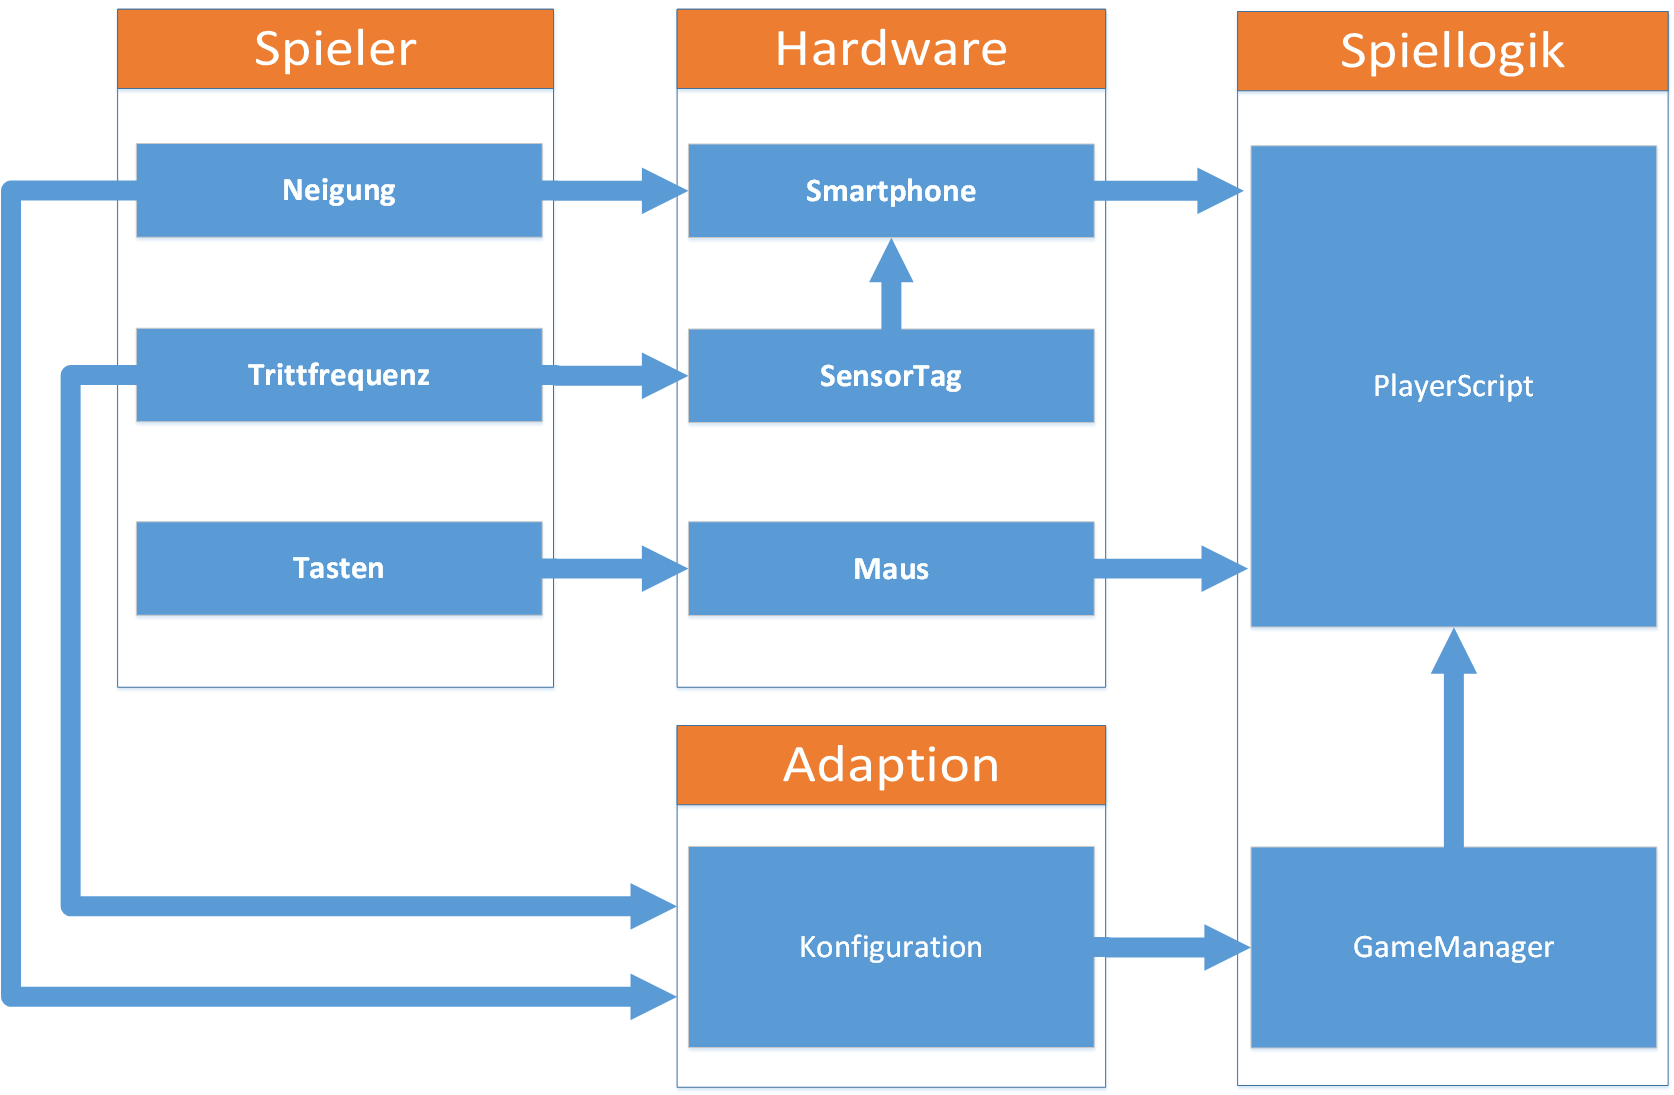
\includegraphics[width=.7\textwidth]{gfx/Steuerung.png}
\caption{Zusammenspiel der verschiedenen Steuerungskomponenten}
\label{Steuerung}
\end{figure}
\section{Steuerung}
Zu den wichtigsten Skripten gehört das \texttt{PlayerScript}. Dieses verarbeitet die verschiedenen Eingaben des Spielers und wandelt diese in Bewegungen um. Je nach Konfiguration wird entweder die Steuerung per Fahrradergometer oder zu Testzwecken die Steuerung per Tastatur verwendet.\\
Die Daten für die Steuerung per Fahrradergometer werden vom \texttt{SensorDataReceiver}-Skript erfasst, indem dieses ein UDP-Socket erstellt, mit dem sich dann das Smartphone verbindet. Das Parsing der Daten erfolgt ebenfalls in diesem Skript.
\section{Leveleditor}
Von Anfang an war klar, dass eine große und abwechslungsreiche Anzahl an Levels für ein gut funktionierendes Spiel wichtig ist. Zuerst war die Idee, diese Levels direkt in Unity als einzelne Szenen zu bauen, doch das erschien uns zu umständlich. Aber selber einen vollständigen Leveleditor zu bauen, hätte wohl den Umfang des Projektes gesprengt.\\
Die Lösung war, einfache Textdateien zu nutzen, und somit einen Texteditor zum Leveleditor zu machen. Die Idee ist dabei, dass jeweils ein Zeichen eine Zelle des Levels füllt. Je nachdem, welches Zeichen dann dort steht, erscheint an dieser Stelle der ein oder andere Baustein, oder es bleibt eine Lücke. Ein Beispiel eines solchen Levels ist in Abbildung \ref{Leveldatei} zu sehen.\\
\begin{wrapfigure}{r}{5.6cm}
\centering
\begin{tabular}{|l|}
\hline
\texttt{25}\\
\texttt{...g...}\\
\texttt{...l...}\\
\texttt{...l...}\\
\texttt{...l...}\\
\texttt{...L...}\\
\texttt{...L...}\\
\texttt{...r...}\\
\texttt{..ftf..}\\
\texttt{...ll..}\\
\texttt{....l..}\\
\texttt{....ll.}\\
\texttt{.....s.}\\
\hline
\end{tabular}
\caption{Beispiel für eine Leveldatei}
\label{Leveldatei}
\end{wrapfigure}
Die Bedeutung der verschiedenen Buchstaben wird im Inspektor des Unity-Editors konfiguriert. Hierbei wird jedem Buchstaben ein Prefab zugewiesen, also ein vorgefertigtes Spielobjekt inklusive eventueller Skripte, die das Verhalten beeinflussen.\\
Ein Buchstabe ohne Zuordnung verursacht dabei keinen Fehler, sondern wird als Lücke interpretiert. Die Konvention ist jedoch, dass nur Punkte für Lücken benutzt werden. Die von uns im Spiel gewählte Zuordnung ist die Folgende:
\begin{itemize}
\item \texttt{l}: Einfacher Streckenabschnitt
\item \texttt{s}: Spieler-Startposition
\item \texttt{g}: Ziel des Levels (Goal)
\item \texttt{t}: Strecke mit Tunnel
\item \texttt{r}: Rampe
\item \texttt{b}: Quadratischer Block in der Mitte des Abschnitts
\item \texttt{f}: Block der über die ganze Breite und Länge des Abschnitts geht
\end{itemize}
Großbuchstaben werden genau wie der entsprechende Kleinbuchstabe behandelt, jedoch wird das Prefab einige Einheiten weiter oben instanziiert, sodass man mittels Klein- und Großbuchstaben Level mit zwei Höhenebenen bauen kann. Die Zahl in der ersten Zeile wird gesondert gelesen und gibt die maximale Leveldauer in Sekunden an.
\section{Szenen}
Auch wenn die einzelnen Level nicht als Szenen realisiert sind, so gibt es dennoch mehrere Szenen im Spiel. Diese sind mit den Szenenübergängen in Abbildung \ref{Szenen} visualisiert.\\
\begin{figure}[ht]
\centering
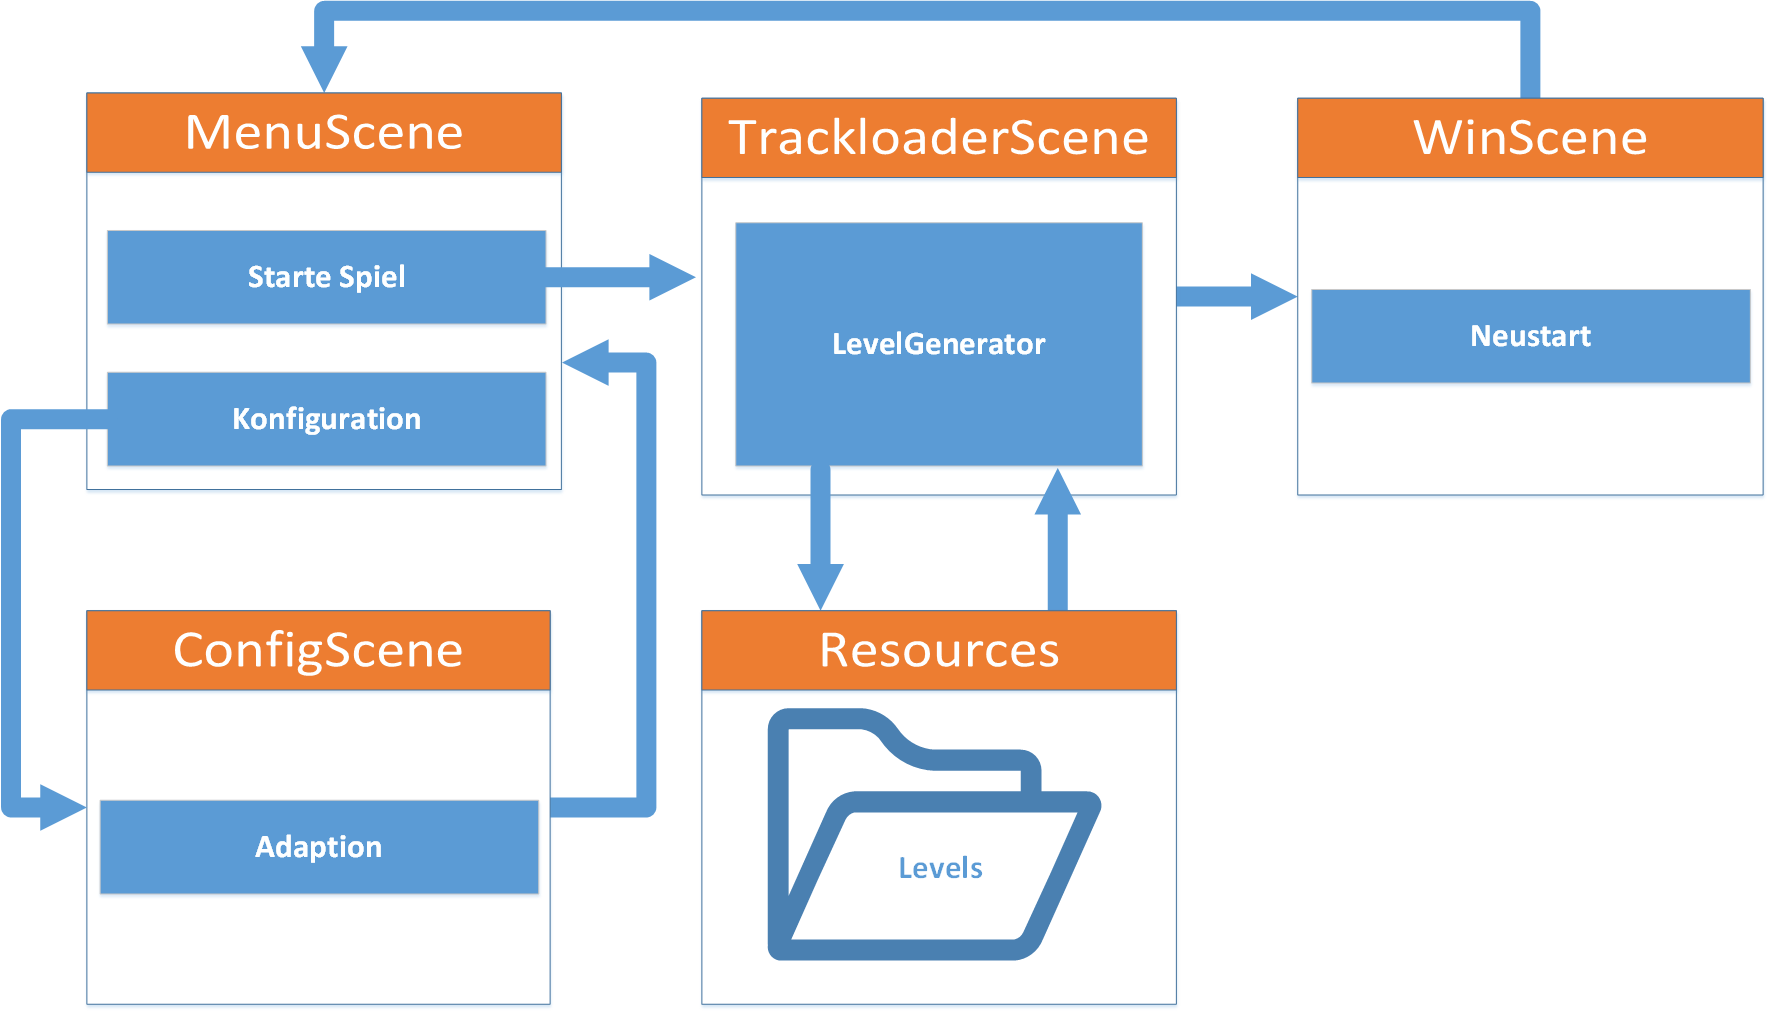
\includegraphics[width=.7\textwidth]{gfx/Szenen.png}
\caption{Szenen und Übergänge}
\label{Szenen}
\end{figure}

\chapter{Anleitung}
\label{Anleitung}

\section{Konfiguration}
In der Konfiguration kann man verschiedene Einstellungen für das Verhalten des Spiels vornehmen.

\begin{figure}[h]
  \begin{center}
    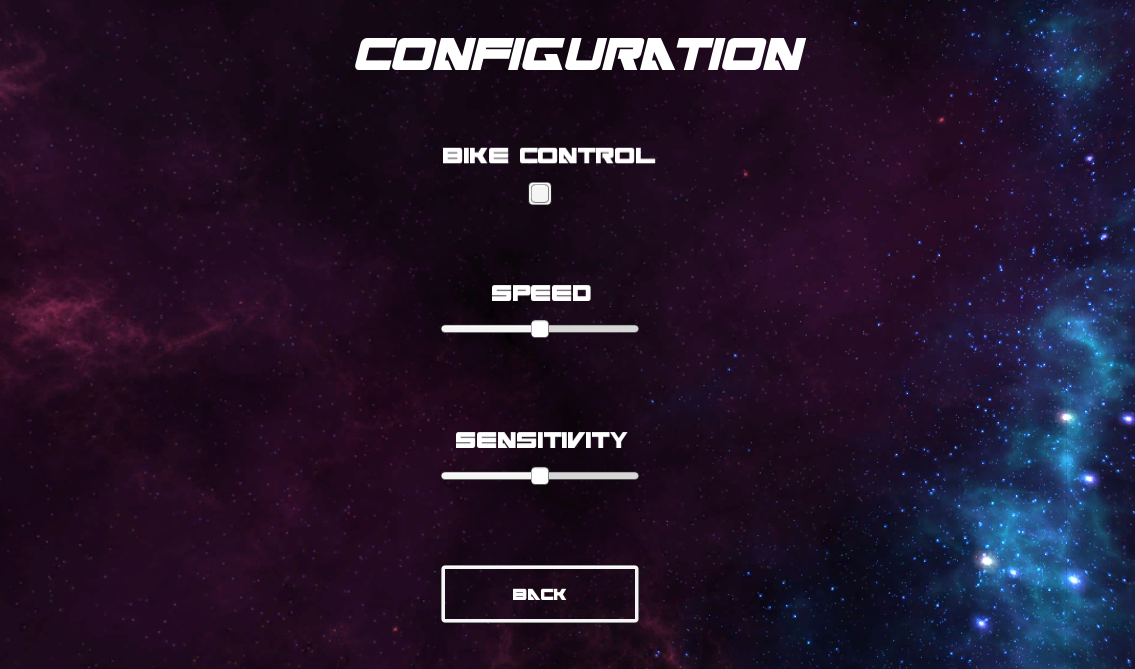
\includegraphics[width=.9\textwidth]{gfx/anleitung/config.png}
    \caption{Konfiguration}
  \end{center}
\end{figure}

\begin{itemize}
  \item \textbf{Bike Controls} \\
  Ist diese Option ausgewählt, kann das Spiel mit Hilfe des Ergometers gesteuert werden, anderenfalls steuert man das Raumschiff mit den Pfeiltasten auf der Tastatur, sowie der Leertaste.
  \item \textbf{Speed} \\
  Diese Option bietet die Möglichkeit die Geschwindigkeit des Ergometers anzupassen. Standardmäßig befindet sich der Geschwindigkeitsmodifikator auf einem mittleren Wert. Um die Geschwindigkeit anzupassen kann der Wert entweder verringert oder erhöht werden. Ein höherer Wert des Reglers bedeutet eine schnellere Geschwindigkeit, ein niedriger Wert entsprechend eine langsamere Geschwindigkeit.
  \item \textbf{Sensitivity}\\
   Diese Option beeinflusst, ähnlich wie die Geschwindigkeit, die Sensitivität des Ergometers. Je nach Einstellung des Reglers reagiert das Fahrrad leichter oder schwerer. Wird der Regler auf einen hohen Wert eingestellt reagiert das Ergometer mehr auf Veränderungen der Neigung. Ein niedriger Wert senkt die Sensitivität entsprechend.
  \item \textbf{Back} \\
  Durch drücken des Buttons \textit{Back} werden die Einstellungen gespeichert und man gelangt ins Hauptmenü zurück.
\end{itemize}

\section{Steuerung}
Das Spiel besitzt zwei Möglichkeiten der Steuerung: Tastatur- und Ergometersteuerung. Bei beiden Varianten kann jeweils zusätzlich die Maus genutzt werden. \\

\subsection{Tastatursteuerung}
Ist in der Konfiguration nicht die Steuerung mittels Ergometer aktiviert gilt folgende Tastenbelegung.

\begin{itemize}
  \item \textbf{Pfeiltaste Hoch:} Erhöht die Geschwindigkeit des Raumschiffes.
  \item \textbf{Pfeiltaste Runter:} Verringert die Geschwindigkeit des Raumschiffes.
  \item \textbf{Pfeiltasten Links/Rechts:} Steuerung des Raumschiffes nach Links oder Rechts.
  \item \textbf{Leertaste:} Lässt das Raumschiff springen.
  \item \textbf{Rechte Maustaste:} Neustart des aktuellen Levels
  \item \textbf{Escape:} Zurück zum Hauptmenü.
\end{itemize}

\subsection{Ergometersteuerung}
Ist die Ergometersteuerung eingeschaltet gibt es folgende Eingabemöglichkeiten.

\begin{itemize}
  \item \textbf{Trittfrequenz erhöhen:} Erhöht die Geschwindigkeit des Raumschiffs.
  \item \textbf{Trittfrequenz verringern:} Verringert die Geschwindigkeit des Raumschiffes.
  \item \textbf{Neigung des Ergometers nach Links/Rechts:} Steuerung des Raumschiffes nach Links oder Rechts.
  \item \textbf{Linke Maustaste:} Lässt das Raumschiff springen.
  \item \textbf{Rechte Maustaste:} Neustart des aktuellen Levels
  \item \textbf{Escape:} Zurück zum Hauptmenü.
\end{itemize}

\section{Spiel}
Hat der Benutzer das eigentliche Spiel gestartet findet er diverse Informationen vor, die ihm ein Feedback über den aktuellen Status des Spiels vermitteln sollen. Die einzelnen Objekte und Anzeigen werden nachfolgend erläutert.

\begin{enumerate}
  \item \textbf{Levelanzeige} \\
   Diese Anzeige zeigt die Nummer des aktuellen Levels an.
  \item \textbf{Fortschrittsanzeige} \\
  Hier wird der Fortschritt im akutellen Level angezeigt. Je voller der Balken ist, desto weiter fortgeschritten ist der Spieler.
  \item \textbf{Spielfigur} \\
  Die durch den Spieler gesteuerte Figur. Die Düsenantriebe geben zusätzlich ein Feedback über die aktuelle Geschwindigkeit.
  \item \textbf{Kraftstoffanzeige}\\
  Hier erkennt der Spieler den verbleibenden Kraftstoff. Verbleibender Kraftstoff symbolisiert die Zeit, die dem Spieler bleibt das Level zu beenden. Je voller der Kreis ist, desto mehr Kraftstoff verbleibt dem Spieler. Ist der Kraftstoff aufgebraucht gilt das Level als verloren und der Spieler muss das Level von Vorne beginnen. Das Raumschiff beginnt Kraftstoff zu verbrauchen, sobald es zum ersten mal beschleunigt wird.
  \item \textbf{Geschwindigkeitsanzeige}\\
  Zeigt die aktuelle Geschwindigkeit an. Befindet sich das Raumschiff im Stillstand ist die Anzeige leer, hat der Spieler die maximale Geschwindigkeit erreicht ist die anzeige komplett gefüllt. 
  \item \textbf{Bahn} \\
  Die Bahn ist das eigentliche Level. Der Spieler darf nicht von ihr abkommen, sonst muss er das Level neu beginnen. Am Ende der Bahn befindet sich ein Zielbereich. Erreicht er das Ziel bevor ihm der Treibstoff ausgeht hat er das Level erfolgreich beendet. Die Bahn kann neben der normalen Fahrbahn aus verschiedenen Objekten und Hindernissen bestehen. Beispiele hierfür sind Tunnel, Rampen oder verschiedene Blöcke, die in späteren Leveln nach und nach eingeführt werden.
\end{enumerate}

\begin{figure}
  \begin{center}
    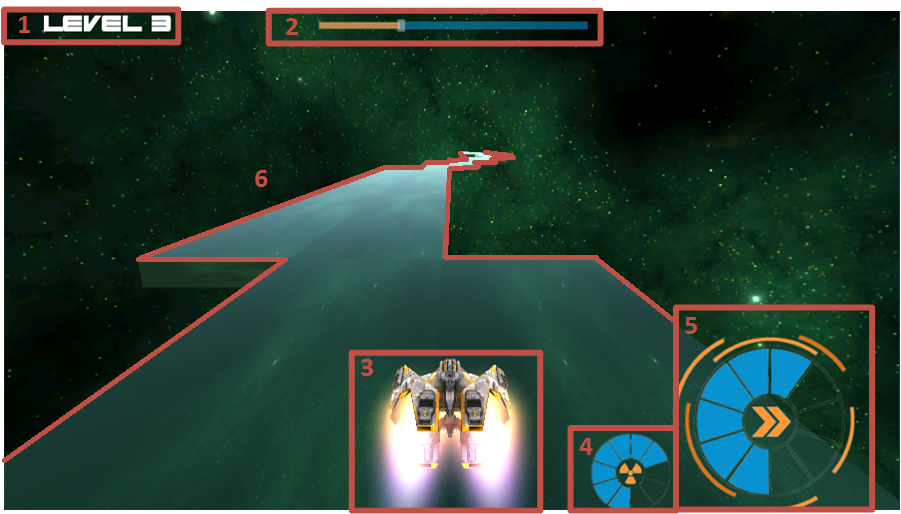
\includegraphics[width=.9\textwidth]{gfx/anleitung/ingame2.png}
    \caption{Spielansicht}
  \end{center}
\end{figure}


\chapter{Zusammenfassung und Ausblick}
Das Ziel des Projektes war es, ein Spiel zur Förderung des Trainings des Oberkörpers auf einem Fahrradergometer zu konzipieren und umzusetzen. Hierfür wurde zunächst eine umfassende Recherche möglicher Spielideen und der Hardware durchgeführt. Anhand dieser Recherche konnte ein Spielkonzept inklusive Spielbeschreibung erstellt werden. Die entsprechende Umsetzung wurde in weiteren Schritten geplant und dokumentiert, bevor die eigentliche Implementierung begonnen wurde. \\
Bei der Umsetzung konnten sämtliche geplanten Features realisiert und getestet werden, dennoch bietet das in diesem Praktikum abgeschlossene Projekt einige Möglichkeiten zur Erweiterung der Funktionalität. Es wäre zum Beispiel denkbar dem Spieler zusätzliche Anreize innerhalb der Level zu bieten. So könnte man bestimmte Objekte auf den Bahnen platzieren durch welche der Spieler Vorteile innerhalb des aktuellen, beziehungsweise der nächsten Levels hat oder wodurch der Spieler neue Fähigkeiten und/oder Objekte freischalten kann. \\
Eine weiter Möglichkeit das Spiel stetig zu erweitern bietet der realisierte Leveleditor. Durch die einfache Integration in das Projekt können zukünftige Entwickler mit sehr geringem Aufwand neue Level-Objekte erstellen und dadurch den Umfang des Spieles schnell erheblich vergrößern. Ebenfalls mit Hilfe des Leveleditors können schnell neue Levels erstellt werden, die anschließend durch die verschiedenen Texturen und Hintergründe nach bestimmten Themen sortiert werden können. Es wäre zum Beispiel denkbar ein Thema mit stark erhöhter Gravitation zu erstellen, welches sich über eine gewisse Anzahl von Levels erstreckt. Dadurch können, ohne dass neue Spielobjekte oder -mechaniken erstellt werden müssten neue Anreize gesetzt werden.\\
Um den kompetetiven Gedanken der Spieler zu fördern wäre eine Highscoreliste dienlich. Statt dem einzigen Ziel das Spiel erfolgreich zu beenden, könnte man zusätzlich Faktoren wie zum Beispiel benötigte Zeit, benötigte Versuche, verbleibende Energie, oder andere in einer Liste speichern. Hierfür sind jedoch noch weitere Anpassungen notwendig, um die genannten Faktoren erfassen und speichern zu können.\\
Die wohl weitreichendsten Änderungen könnten jedoch mit der Personalisierung des Spieles an den Spieler erreicht werden. Zwar bietet das Projekt zum jetzigen Stand bereits die Möglichkeit die gemessene Geschwindigkeit und die Sensitivität des Ergometers an den jeweiligen Spieler anzupassen, allerdings werden diese Einstellungen noch nicht gespeichert. Denkbar hierfür wäre eine Art Benutzerverwaltung, in der verschiedene Spieler ein Profil hinterlegen können, welches ihre Einstellungen speichert. Im Zuge dessen könnte ebenfalls der Spielfortschritt gespeichert werden. \\
Zusammenfassend kann man festhalten, dass im Rahmen dieses Praktikums ein Bewegungsspiel konzipiert und implementiert wurde, dass alle relevanten Punkte der Aufgabenstellung erfüllt und darüber hinaus zusätzlich noch sehr viel Raum für eventuelle weitere Entwicklungsschritte bietet. Durch die realisierten Adaptionsmechanismen eignet sich das Spiel für eine große Bandbreite von Zielgruppen und besitzt dabei das Potenzial spielerisch zur Gesundheitsförderung beitragen. Dieser Aspekt sollte in naher Zukunft durch eine Benutzerstudie evaluiert werden.

